% !TEX encoding = UTF-8
% !TEX TS-program = pdflatex
% !TEX root = ../Volpe_Andrea.tex

%**************************************************************
\chapter{Ristrutturazione database}
\label{cap:ristrutturazione-database}
%**************************************************************

\intro{In questo capitolo viene descritta la fase di ristrutturazione del database per
la realizzazione del progetto.}
\\\\\\\\\\\\
Durante la fase di studio del database ho rilevato la presenza di
alcune criticità che hanno richiesto una revisione della base di dati.
\\\\
Attraverso il confronto con un'altro stagista con il quale si condivideva la stessa base di dati 
è emersa la necessità di una revisione del modello logico.
\\\\
Rilevate le criticità abbiamo verificato che il database fosse in forma normale, in quanto una base 
di dati non in forma normale presenta problemi di ridondanza, inefficienza, complessità e perdita di 
informazioni.
\\
Un database è in forma normale se soddisfa le tre forme:
\\
\begin{itemize}
  \item La prima forma normale dice che le tabelle non contengono gruppi (colonne) ripetuti;
  \item La seconda forma normale dice che tutti gli attributi di una tabella dipendono dalla chiave completa;
  \item La terza forma normale dice che nessuna colonna di una tabella è dipendente da una colonna descrittore, 
  che a sua volta dipende dalla chiave primaria.
\end{itemize}
\leavevmode\newline
Il database soddisfava le tre forme ed era quindi in prima, seconda e terza forma normale ma presentava comunque criticità che hanno richiesto 
una ristrutturazione.
\\\\
Una revisione o modifica di un database all'interno di progetti ha impatti importanti, in questo
particolare caso sono stati coinvolti tutor aziendale e sviluppatori interessati per condividere
l'intervento. 
\\\\
Lavorando su branch indipendenti si sono riuscite a mantenere le modifiche 
in isolamento senza impatti, riuscendo a testare la correttezza dell'intervento in una base di dati locale.
\\\\
Successivamente l'azienda valuterà in fase di rilascio le versioni adeguate da installare
negli ambienti di sviluppo collaudo ed esercizio.
\\\\
\clearpage
Il modello logico esistente era il seguente:
\begin{figure}[H]
  \centering
  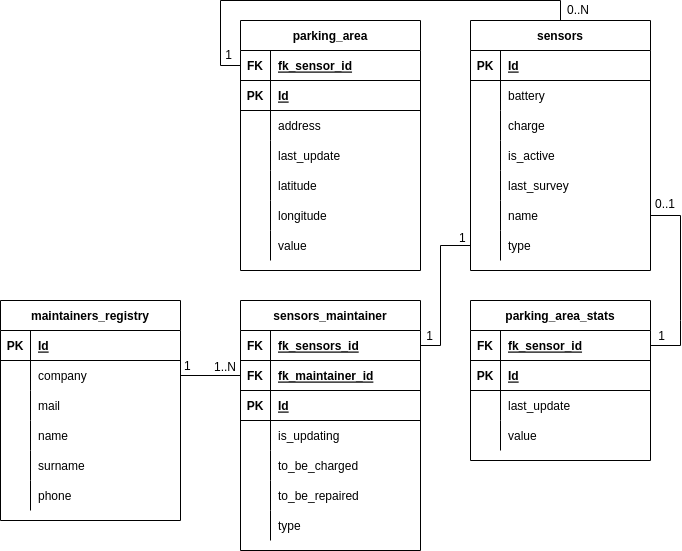
\includegraphics[height=8cm]{modello-logico-vecchio}
  \caption{Modello logico pre-ristrutturazione}
\end{figure}

\section{Anomalie rilevate}
Partendo dalla premessa che il software è un prodotto in continua evoluzione, le prime versioni
di prodotto possono presentare anomalie o bug.
\\\\
La stessa progettazione del modello logico iniziale può possedere mancanze, lacune oppure subire variazioni da nuovi requisiti. 
\\
I framework di persistenza (es. JPA) 
riescono a facilitare questo tipo di interventi correttivi.
\\
Seguono una serie di anomalie rilevate e di adeguamenti eseguiti rispetto alla prima versione del modello dati:
\\\\\\
\textbf{Nomi tabelle incoerenti}
\\\\
I nomi di alcune tabelle erano incoerenti con la funzionalità che svolgevano:
\\\\
sensors\_maintainer era la tabella contenente i dati di manutenzione dei sensori, un 
nome più appropriato poteva essere sensors\_maintenance.
\\\\
parking\_area era la tabella rappresentante la piazzola di parcheggio, un nome più appropriato
poteva essere parking\_spots.
\\\\\\
\clearpage
\leavevmode\newline
\textbf{Duplicazione di dati}
\\\\
La tabella parking\_area\_stats non serviva, in quanto duplicava dei dati già presenti
nella tabella parking\_area, creando un'inutile ridondanza.
\\\\\\
\textbf{Cardinalità delle relazioni errata}
\\\\
La relazione sensors -> parking\_area aveva cardinalità uno a molti, nel senso che una piazzola poteva avere
più sensori e un sensore poteva essere associato solo a una piazzola. 
\\
Questa logica è errata, in quanto è vero che una piazzola potrebbe avere più sensori associati (un sensore di parcheggio e/o N
sensori ambientali) ma anche un sensore può essere associato a più piazzole; in quanto un sensore ambientale
potrebbe ricoprire un area di N piazzole.
\\\\\\
\textbf{Mancanza di tabelle fondamentali}
\\\\
Mancava una tabella fondamentale che rappresentasse un parcheggio (un insieme di piazzole). 
\\
Tabella molto importante dato che un parcheggio ha un indirizzo e una posizione geografica (latitudine e longitudine), 
riconosciute come tali dagli strumenti di navigazione più comuni, come Google Maps. 
\\
Ogni piazzola di uno stesso parcheggio ha una posizione geografica diversa dalle altre piazzole (discostata di qualche 
metro) e potenzialmente diversa da quella del parcheggio. 
\\
Con la struttura vecchia non era possibile ricercare un parcheggio a sistema passando le coordinate del parcheggio di Google
Maps ad esempio e nemmeno identificare un singolo parcheggio.
\\\\\\
\textbf{Database poco modulare}
\\\\
La misurazione del sensore di parcheggio veniva salvata all'interno di un campo della tabella parking\_area (libero/occupato). La cosa non creava problemi con il modello progettuale dove,
dall'analisi fatta, si era deciso di salvare solo l'ultima misurazione di un sensore di parcheggio.
\\\\
Se però in futuro si decidesse di salvare uno storico di misurazioni dei sensori di parcheggio (cosa molto probabile che
avvenga e cosa che già viene fatta con i sensori ambientali), non sarebbe possibile farlo e i costi
per modificare la struttura del database con il software in esercizio su un ambiente di produzione, sarebbero molto più
alti rispetto a farlo in fase di sviluppo.
\\\\
Inoltre l'aggiunta di una tabella per lo storico non ha un impatto negativo sulla struttura del database.
\clearpage
\section{Ristrutturazione}

Il modello logico ristrutturato è il seguente:
\begin{figure}[H]
  \centering
  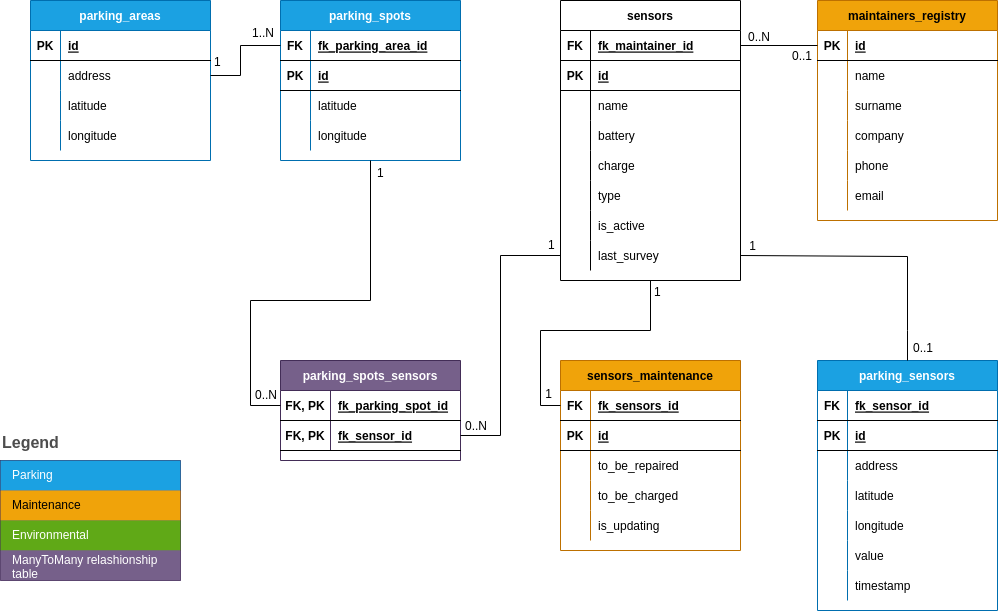
\includegraphics[height=8cm]{modello-logico-ristrutturato}
  \caption{Modello logico post-ristrutturazione}
\end{figure}
\leavevmode\newline
\textbf{Operazioni effettuate:}
\\\\
\textbf{Nomi tabelle incoerenti}
\\\\
Sono stati modificati i nomi di alcune tabelle per renderle coerenti alla loro funzionalità:
\\\\
parking\_area è stata modificata in parking\_spots.
\\
sensors\_maintainer è stata modificata in sensors\_maintenance.
\\\\
\textbf{Duplicazione di dati}
\\\\
E' stata eliminata la tabella parking\_area\_stats.
\\\\
\textbf{Cardinalità delle relazioni errata}
\\\\
La relazione sensors -> parking\_area è diventata una relazione molti a molti.
\\
E' stato reso facoltativo che il sensore debba essere associato a una piazzola.
\\
E' stato reso facoltativo che il manutentore debba essere associato a un sensore.
\\
E' stato reso facoltativo che il sensore debba essere associato a un manutentore.
\clearpage
\leavevmode\newline
\textbf{Mancanza di tabelle fondamentali}
\\\\
E' stata aggiunta la tabella parking\_areas in rappresentanza dei parcheggi, dotati di indirizzo, latitudine e 
longitudine.
\\\\
\textbf{Database poco modulare}
\\\\
E' stata creata la tabella parking\_sensors per salvare la misurazione del sensore di parcheggio ed è
stato rimosso il campo value dalla nuova tabella parking\_spots; in quanto con la tabella parking\_sensors,
rappresentava una ridondanza inutile.
\\\\
Per ogni sensore di parcheggio viene salvata solo una misurazione nella tabella parking\_sensors, ovvero
l'ultima, sovrascrivendo la precedente ma a differenza del modello logico precedente, se 
si decidesse di salvare lo storico delle misurazioni dei sensori di parcheggio, sarebbe sufficiente rimuovere
il vincolo unique dalla foreign key \textit{fk\_sensor\_id} della tabella parking\_sensors, senza modificare la struttura della base di dati.